% Chapter 3
\setcounter{tocdepth}{4}

\chapter{State of the Art} % Main chapter title
%\epigraph{A fancy quote}{Me}

\label{art} % For referencing the chapter elsewhere, use \ref{Chapter2} 

\lhead{Chapter 3. \emph{State of the Art}} % This is for the header on each page - perhaps a shortened title

This chapter provides a review of the literature, introduce basic concepts and reviews the techniques most used to solve this kind of problems. It is divided into two main sections. In the first section techniques used in the scientific literature are explored. The second section gives a technological overview. This last section is important because it shows the difference between studying practical applications that solve real-world timetabling problems against simplified models of the reality.
%----------------------------------------------------------------------------------------

\section{Scientific Overview}

Over the past decades, a large number of techniques has been applied to timetabling problems with varied success. Although there is no accepted solution yet that can globally solve the problem, mainly because each institution has its own requirements, there are many interesting approaches to tackle the problem. In this section we make a little survey of algorithms. We also present some benchmarks works useful to determine which techniques are in general the best computational methods. 
\subsection{Approaches to Automated Timetabling}

There are a very wide range of approaches to the timetabling problem. These approaches may then be broken down in a large variety of techniques. Figure \ref{fig:techniques} shows a conceptual model of the existing techniques.

\begin{figure}[th]
	\centering
	    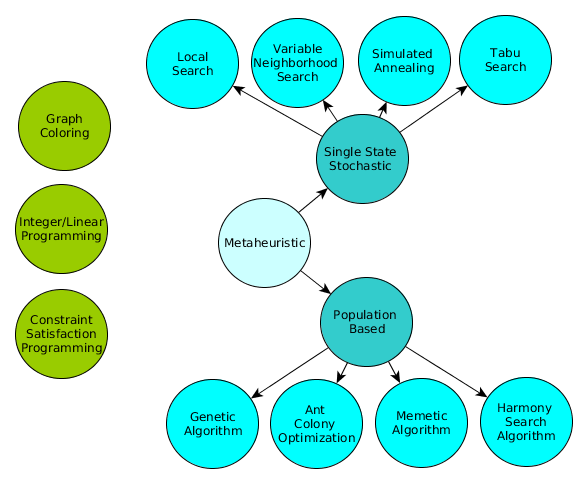
\includegraphics[scale=0.5]{./Figures/DataStructures/yED/techniques.png}
	\rule{35em}{0.5pt}
	\caption[Techniques Applied to the University Timetabling Problem]{Techniques Applied to the University Timetabling Problem} 
	\label{fig:techniques}
\end{figure}

Lewis \citep{lewis2008survey} distinguish approaches based on how the algorithms attempt to solve the two kind of constraints, i.e, hard and soft constraints. Regarding this matter, they usually fall into one of the two categories:
\begin{itemize}
	\item{\textbf{One-Stage Optimization Algorithms}} - The satisfaction of both hard and soft constraints is attempted simultaneously. In this case the violation of hard and soft constraints is allowed and the quality of a solution is measured through a typical weighted sum function, where the penalties for hard constraints are much higher when compared to violations of soft constraints. 
	\item{\textbf{Two-Stage Optimization Algorithms}} - The satisfaction of soft constraints is only attempted once feasibility is found, i.e., all of the hard constraints are solved. This has the immediate advantage of only considering weights for soft constraints and applying search techniques only in feasible areas, i.e, using classical search improvement procedures to move from old solutions to better solutions.
\end{itemize}

Carter and Laporte \citep{recent_dev_patat} extends this idea and also consider the existence of constructive heuristics, i.e, algorithms where sequential assignments are made while preserving feasibility, until is no longer possible to make assignments (due to violations). Then some backtracking procedures are applied in order to undo the changes and restart the sequential assignment process.

The next list shows a survey of related works under the categories presented in Figure \ref{fig:techniques}:

\paragraph{\textbf{Graph Coloring}} - The problem of coloring a graph with a set of colors such that no two adjacent vertices share the same color is a classic assignment problem. De Werra \citep{introduction_timetable} used this technique to solve the class-teacher timetabling problem. Basically, he described a bipartite multi-graph in which the nodes are the teachers and the classes and the edges represent a relation between a teacher and a class. Thus, two nodes may be linked by a number of parallel edges, depending on how many classes involving a teacher and a class are there. The problem is then reduced to finding an assignment of one among \textit{p} colors (timeslots) to each edge in such a way that no two adjacent edge share the same color. Another way of stating the problem is that of finding a set of \textit{n} matchings, attributing the same color to all the edges of the same matching (by definition, in a matching there are no adjacent edges) such that the final graph does not have adjacent edges with the same color. De Werra showed previously that is possible to find such matchings using network flow techniques \citep{deWerra}. 
	Figure \ref{fig:bipartite} despises this situation.\par
	  \begin{minipage}{\linewidth}
            \centering
            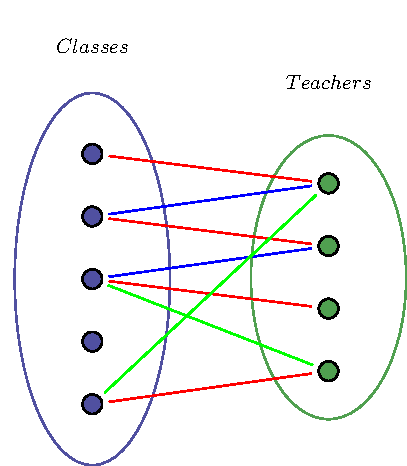
\includegraphics[scale=0.7]{./Figures/tkiz/bipartite.pdf}
            \captionof{figure}{Bipartite colored matching}
            \label{fig:bipartite}
        \end{minipage}
By using the graph coloring, Karich and Bahurmoz \citep{peter_karich},\citep{bahurmozhungarian} are able to assign events to rooms and time slots efficiently. Essentially, they use the Hungarian algorithm to find perfect matchings, i.e, matchings that minimize certain costs. The Hungarian algorithm is an algorithm that solves the assignment problem in polynomial time and is used to achieve perfect matchings that minimize the assignment costs. In this case the costs may be related to the quality of associating an event to a room or to a time slot.
    The most simple timetabling problem can be converted to a graph coloring, by considering each vertex as an event and edges representing conflicts (e.g.: cannot be assigned in the same time slot). Each color represents then a time slot and the problem is now to find an assignment of colors to vertices that used no more than the available colors. Another way of seeing the problem is to determine the minimum number of colors needed in order to avoid collisions between events, but unfortunately it is also an NP-hard problem. Nearly all timetabling problems have this underlying graph coloring problem.

\paragraph{\textbf{Integer/Linear Programming}} - Linear programs are methods used for optimizing outcomes of mathematical models, i.e, maximizing or minimizing costs. Usually, there is an objective function to be maximized or minimized. This function is also subject to some constraints usually expressed in the form of mathematical inequalities. When only integers are allowed for the values of the variables, it is called integer programming. A variant commonly used in solving timetabling problems is called 0-1 integer programming where the variables have binary values. For instance, Daskalaki and Birbas \citep{daskalaki2005efficient} developed a two-stage relaxation procedure to solve efficiently an 0-1 integer formulation of the problem. In their work, some hard constraints are relaxed (not considered) in the first stage and recovered in a second stage. In terms of formulation, they reuse the work performed in \citep{daskalaki2004integer} and they consider the possible assignment of a lecture, taught by a teacher to a set of students, scheduled in a period of day and in a classroom as a single variable that may have the value 1 (the assignment is performed) or 0 (the assignment is not performed). They later define an objective function subject to a set of formulated constraints and this optimization helps minimizing the total cost of the assignments. A downside of this approach is that introduces too many variables as the problems grows in size. On the other hand, it brings a great flexibility in terms of adapting the constraint formulations and the objective function to different requirements of different institutions.

\paragraph{\textbf{Constraint Satisfaction Programming}} - Timetabling problems may be modeled as set of clauses in which each clause has a body with constraints. Besides a set of discrete variables with discrete domains are also defined. Therefore it is possible to formulate a combinatorial problem such assigning events to time slots in terms of variables and their domains and a set of constraints that constraint the assignment of values to these variables. In constraint satisfaction programs, the objective is to find a set of values that satisfy a set of constraints. Usually this technique is followed by \textit{"forward checking"} which allows to determine the effects of assigning a value to a variable. This means that each time a variable is chosen, every other possible  assignment from another variable that is not consistent with that new assignment is eliminated from the respective domains. This brings an advantage because it decreases the search space. Besides, CSP programs have the logic separated from the control, i.e, the declaration of variables and constraints is separated from the information regarding the search strategies to follow. In fact, the university of Leeds \citep{leed_clp} developed a Prolog system based on Constraint Logic Programming (an application of logic programming languages to CSP).

\paragraph{\textbf{Local Search}} - Local search techniques consider solutions that move in the search space by exploiting several different neighborhoods. Usually, the search starts in an initial solution and iterates over the search space, steping from one solution to one of its neighborhoods. Therefore, neighborhoods are core structures of this approach and a good definition of a set of operators that create neighborhoods are usually an important part of the process. Each neighborhood is obtained by applying small "changes" called moves to solutions. Di Gaspero and Schaerf \citep{di2003multi} performed an extensive study of neighborhood structures applied to the timetabling problem. They investigate three main kind of neighborhood combinations:
	\begin{itemize}
		\item Neighborhood Union - For example, two basic resources in timetabling are time slots and rooms. Thus, by simply changing a room of a lecture or a time slot of a lecture two new neighborhoods are defined. The union operator, at each iteration of the search procedure, performs one of these moves.
		\item Neighborhood Composition - In this case, an ordered sequence of moves belonging to different neighborhoods is performed.
		\item Token-ring search - This technique performs a circular search through all the neighborhood operators and it always stars from the best solution found in the previous search.
	\end{itemize}
	Another common technique used is the Iterated Local Search and Roosi-Doria et al. \citep{rossi2003comparison} used this technique where small perturbations are made to the timetables in order to search in new promising areas. 

\paragraph{\textbf{Variable Neighborhood Search}} - Variable neighborhood search usually uses more than one neighborhood structure where those structures may change during the local search. Abdullah et al. \citep{abdullah2005investigation} use an acceptance criteria similar to simulated annealing but without a cooling schedule. The motivations was to search new points of the search space. In terms of neighborhood moves, they implemented twelve different operators in which some of them simply move a lecture (obtained from a random sample of varying size of assigned lectures) to a new feasible time slot. The algorithm followed an iterative three stage approach where first a random solution is obtained followed by a local search and then the new solution is accepted based on a acceptance criteria. As highlighted by the authors, the order of neighborhoods that gave the best results was when the neighborhood structures were ordered in an increasing size, i.e, with a bigger number of possible moves. This way solutions could go smoothly from local searches to more global searches.
  

\paragraph{\textbf{Simulated Annealing}} - Simulated annealing is a search strategy inspired  in the slow annealing process in metallurgy. The difference from a simple Hill Climbing algorithm is in its decision of when to replace a solution, i.e, a newly tweaked solution may be accepted even if it is worse than the current solution, according to a certain probability. This probability is controled by a parameter called temperature and the rate at which this value is changed is called the cooling schedule. Aycan and Ayav \citep{aycan2009solving} use a simulated annealing approach to solve the timetabling problem.  This approach is a very problem dependent because it needs a suitable cooling schedule and good neighborhood structures. In order to create neighborhoods, random lectures were given new time slots or two lectures had their time slots swapped or two random lectures were assigned to two new random time slots.

\paragraph{\textbf{Tabu Search}} - Tabu search is a search procedure that keeps an history of moves that led to better solutions (a tabu list), i.e, usually a solution that is obtained by applying repeated moves from the past is avoided, preventing cycles. This avoid locking solutions in suboptimal regions, like local minima. Tabu search uses a local or neighborhood search procedure to iteratively move from one potential solution to an improved solution in the neighborhood. Tabu search provides intensification and diversification, i.e, it examines thorough the neighborhood of good quality solutions and force the search to unknown regions. For the past ten years, Alvarez-Vald{\'e}s et al. \cite{alvarez2001tabu}  have applied tabu search methods in timetabling problems. They use tabu lists of varying lenght, giving better results than static length lists. Another simple criterion that usually works well, is the aspiration criterion where sometimes, a not so good solution may be accepted, ignoring the moves in the tabu list. 

\paragraph{\textbf{Genetic Algorithm}}- Genetic algorithms are inspired in biological mechanisms and reuse similar concepts such as a population, selection of the fittest when subject to an objective function, recombination and mutation where diversity is created and slowly increases the quality of the population in the long run. Common solution representations include encoded numeric arrays where each cell represents the time slot where each event is going to take place. The evolutionary approach used by Roosi-Doria et al. \citep{rossi2003comparison} used this representation with an additional matching algorithm to determine the best suitable room. Such simple representations allows to use crossover and mutation operators (for example, inheriting, in a uniform way, time slots from the parents or a simple swap of events). Usually these procedures are followed by local search techniques in order to improve the quality of the solutions. Carrasco and Pato \citep{carrasco2001multiobjective} developed a multiobjective genetic algorithm that deals with two main objectives: the minimization of both types of constraints and the minimization of conflicts between teachers and classes, i.e, the competing aspects of the soft constraints. The chosen representation was a matrix of time slots per rooms where each cell stored the lecture event currently taking place. The population then evolved over the generations  by applying genetic operators. An interesting fact is that the algorithm also kept a secondary elitist population where the best candidates were saved for the next generation in order to avoid the loss of high-quality solutions. 

\paragraph{\textbf{Ant Colony Optimization}} - Ant colony optimization is another family of optimization algorithms inspired by pheromone-based strategies of ant foraging. The main idea is that ants move randomly in order to find food, while depositing pheromones, leaving a track that becomes stronger as others ants find this track and keep depositing pheromones. There is also a constant phenomenon of evaporation that slowly erases the left pheromones. Roosi-Doria et al. \citep{rossi2003comparison} were the first to apply such technique for a timetabling problem. The method is an iterative process where each ant builds an assignment and keeps a matrix of pheromone values (Time slots $\times$ Events). In order to construct an assignment, an ant chooses the next event from an ordered list and a time slot for that event, based in probabilistic heuristics. Then, it updates the corresponding cell in the pheromone matrix. The probabilistic heuristics were guided by taken into account potential constraint violations and a "rating" of that assignment given by the value of the current pheromone. Besides the pheromones values were constantly being updated after each event assignment and in the end of the iterative process. The iterative process would then keep running for a defined period of time. 

\paragraph{\textbf{Memetic Algorithm}} - Just like genetic algorithms are inspired in biological evolution, memetic algorithms are inspired in the evolution of memes, i.e, symbols or cultural ideas that are transmitted over the generations and may also evolve. The main difference between genes and memes is that memes can be improved by the individual, i.e, memetic algorithms are basically evolutionary algorithms with local optimization techniques. Rossi-Doria and Paetcher \citep{rossi2004memetic} use a classical genetic algorithm with genetic operators (recombination and mutation) to evolve a population but in the end of each iteration, they perform additional local searches. In another work, Paetcher et al. \citep{paechter1996extensions} detail a system in which the local search mechanism consist in suggestion lists of possible time slots, one for each event. The list of events is also permuted in order to place first events with a fewer possibilities first. A mechanism called \textit{searchspec} consists in trying to place an event in each time slot of its suggestion list and if the move is successful, the time slot is moved to the top of the list, improving the memetic material. Other recombination operators are also applied, ensuring that quality ideas are passed over the generations (ancestral memory). 

\paragraph{\textbf{Harmony Search Algorithm}} - Harmony search algorithms are inspired in the process of improvised creation of beautiful harmonies by musicians. Musicians improve the pitches from their musical instruments achieving a pleasant harmony after repeated sessions. In a similar way, a set of decision variables are assigned with values and after repeated iterations, an optimal solution may be found according to an objective function. There are many similarities with genetic algorithms because this technique stores a set of vector variables (solutions) with possible values assigned, just like a typical population, but in this case is called harmony memory. Just like genetic operators, there are operators that change the values of the variables. Finally, by an iterative process the worst vector variable (in terms of quality) is continually replaced by a newly improvised vector, if this one is better. Al-Betar et al.\citep{al2012university} adapted this search procedure to the timetabling problem, by representing a solution as a vector of \textit{n} event variables, where each value maps a room and a time slot (according to a mapping function) for the event represented by the index position. 

\subsection{Standard Formats and Benchmarks}

Usually many different methods are developed to solve the timetabling problems. However, these methods are usually very problem-specific and are only used in a particular institution or research group and are rarely compared with each other. Thus, a problem arises when trying to compare existing methods and determining the best approaches. If a method is simple enough to reproduce, this does not represent much of a problem, but as the complexity of the constraints and techniques grows, comparisons become much harder.\\
Many formats have been developed in order to express in a clear and precise way real-life timetabling problems. Although, the comparison of results and exchange of data between researchers is a difficult process because each one has its own way of formulating the problem. Therefore, the need for a standard format that allows easy exchange of data and testing of algorithms on standards benchmarks have become urgent along the years. Burke et al. \citep{burke1998standard} proposed a functional format for expressing the timetabling problem in a mathematical form. The proposed format was intended for storing data centrally, allowing different researchers to exchange data via this central format.
Currently, the WATT research group also provides datasets from different universities and tools (solutions, verificators, generators and libraries) \footnote{\href{http://www.cs.nott.ac.uk/~yxb/TTdata/}{http://www.cs.nott.ac.uk/~yxb/TTdata/}}.
A good example that promotes the sharing of datasets and testing of algorithms on benchmarks is the International Timetabling Competition \footnote{\href{http://www.utwente.nl/ctit/hstt/itc2011/welcome/}{http://www.utwente.nl/ctit/hstt/itc2011/welcome/}}. The purpose of this competition is for participants to submit algorithms able to solve real world instances of the timetabling problem and then be compared against each other using existing benchmark data. In a very realated work, Roosi-Doria et al. \citep{rossi2003comparison} studied the performance of five different metaheuristics (Evolutionary Algorithms, Ant Colony Optimization, Iterated Local Search, Simulated Annealing and Tabu Search). Both one-stage and two-stage approaches were tried and in general, algorithms with a two-stage approach performed better. Although the performance of the metaheuristics are highly dependent of the context in which they are used, i.e, the solution representation used, neighbourhood search structures, constraints, techniques that used iterated local search offered good results and in many cases outperformed the others.

\section{Technological Overview}

In the following sections we present a small survey of practical approaches currently in use at universities. The technical details of these approaches were gathered from published conference papers, namely the PATAT conference
\citep{leed_clp, purdue_patat_2006, bullet_paper, thor, distributed_timetabling, online_tt_patat2010, diamant}.  

\subsection{Automated Timetabling at the University of Leeds}
At the University of Leeds, the informatics department developed a timetabling engine with a central database capable of storing all of the required information. The implemented algorithm followed an approach based on constraint logic programming \citep{leed_clp}. The used constraints were  formulated in a CLP program.
The implementation consists in several modules that work together. Figure \ref{fig:leeds_workflow} shows the implemented workflow.
\begin{figure}[htbp]
	\centering
		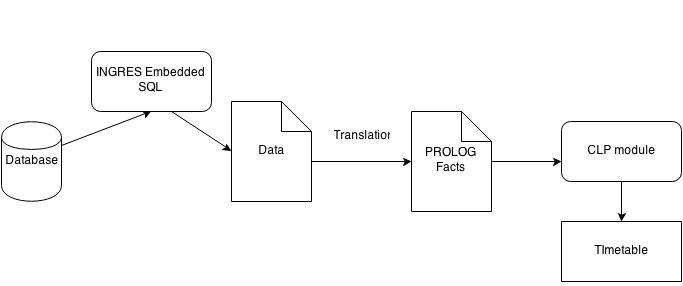
\includegraphics[width=\textwidth]{./Figures/leed_workflow.png}
		\rule{35em}{0.5pt}
	\caption[Implementation workflow of a CLP based system]{Implementation workflow of a CLP based system}
	\label{fig:leeds_workflow}
\end{figure}
 
A SQL script is used to extract the required data from the database. This data is then translated to PROLOG facts. These facts represent the formulation of the problem and will be read by the CLP module. This CLP module is then responsible for generating the timetables.

\subsection{Automated Timetabling in the Purdue University}
In the University of Purdue, a system is being implemented with the main goal of assisting the academic timetablers in constructing a feasible and good timetable \citep{purdue_patat_2006}. The university has large dimensions (9,000 classes, 570 rooms, and 39,000 students) and thus it was necessary to come up with a scalable solution that could deal with the problem.

The developed system consists on 2 different modules:
\begin{itemize}
	\item User Interface - A web-based client-server application written in Java (J2EE) and Hibernate/Oracle Database as the persistence components.
	\item Solver - An engine capable of generating schedules using a Iterative Forward Search approach. This technique is a mixture between local search methods and backtracking because it operates over feasible (not necessarily complete but with all constraints satisfied) solutions.
\end{itemize} 

In terms of features of the application we present a list of interesting aspects:
\begin{itemize}
	\item Interactive changes - If a user wants to change a given class, the interface would provide a list of possible and feasible suggestions (based on a search of limited depth) and the reachable solution cost. The system could also relax some constraints in order to give more freedom to the user when choosing, for example, a room for the class, allowing the user to choose a conflicting room. Of course, if this were the case, all the conflicting events (also shown) would be unassigned. 
	\item Data Consistency - The solver is capable of checking the input for inconsistencies and informing the user about the problem.
	\item Data Management - Possibility of defining preferences and deducing new constraints from these preferences. 
\end{itemize}


\subsection{Bullet TimeTabler Education}
\label{bullet_algorithm}

In Portugal, a company called Bullet Solutions developed a timetabling engine \citep{bullet_paper}.
The followed approach is based on some important principles:
\begin{itemize}
	\item An initial difficulty is to create an initial feasible solution. Therefore, the focus should be on find good methods that allow finding feasible solutions.
	\item The solutions should be found in due time. Therefore, it is important to achieve methods that can quickly cover many areas of the search space. 
\end{itemize}

Given these two principles, the developed algorithm consisted in the following two steps:
\begin{itemize}
	\item Building of an initial solution.
	\item Optimizing the initial solution applying some heuristics. 
\end{itemize}

Initially there is a ordered list of events to be scheduled. The order of criterion is basically the urgency of each event. The urgency of an event is defined by factors like the number of available time slots, the number of available rooms (the lower, the most urgent) or the degree of dependency (through constraints) with other events (the higher, the most urgent).\\ 
This list also contains some redundant events (ghost events) that will not be scheduled in order to increase the flexibility of the algorithm. These ghost events represent the many possible combinations between teachers and turns of a subject. This happens because the algorithm does not consider the association between teachers and their respective turns. In case there are more than one teacher for a given subject, and that subject is taught in more than one turn, there is many possible combinations teacher-turn. Of course if a given event is scheduled, all his complementary ghost events are no longer valid.

After the first feasible solution is found (all events scheduled with hard constraints satisfied), a local search is applied to the solution in order to increase its quality. This search is performed in the neighborhood of the solutions and uses two search operators:
\begin{itemize}
	\item Operator 1 - This operator chooses an event and analyses potential new places to be scheduled. The event may then be moved to these new locations or the events occupying these destination places may be swapped with original event, if possible.
	\item Operator 2 - This operator differs from the first in the swap operation. The destination place is not restricted to the location of the other event. Instead, new locations are possible. 
\end{itemize}

Besides, the software also tries to optimize the use of spaces, i.e., it changes the assigned classrooms in order to optimize the space usage.



\subsection{The THOR System}

The THOR system \citep{thor} was developed by ISEL (Lisbon Institute of Engineering) and is currently commercialized by the company F++, Informática e Serviços. The main objective was to solve the problem of timetabling in Portuguese institutions and to give support to different levels of education (basic, higher, academic,etc). \\
The basic scheduling unit considered is a lesson. A lesson is a triple (T,C,S) in which T is a subset of teachers, C is a subset of classes and S is a subset of subjects. Therefore, a lesson may be simple (when there is only one class and only one subject) or compound (there is more than one class and more than one subject). A compound lesson may have many classes associated with a single subject or a given class associated with many subjects.

The authors made no clear no clear distinction between hard and soft constraints. This problem was solved assigning weights to each constraint and thus allowing different schools assigning different values.


The implementation of the system was divided into three main modules:
\begin{itemize}
	\item A Graphical User Interface - Several forms where it is possible to enter school data and manipulate the schedules.
	\item An automatic scheduler - Developed in C++ using an object oriented approach. The scheduler is capable of following two approaches: An iterative algorithm and a heuristic constructive algorithm. In order to achieve fast evaluations between two neighbor solutions, the cost function is computed incrementally, i.e., the computed value is the difference change in cost between the old solution and the new solution. 
	\item A relational database - Implemented in Microsoft Access.
\end{itemize}

According to the authors, this implementation is currently in use in more than one hundred national schools.

\subsection{A framework for Distributed Timetabling}

At the University of Erlangen-Nuernbergat, efforts have been made in order to come up with a framework that can support all of the timetabling algorithms with optimal parameter settings, \citep{distributed_timetabling}. This requires that all of the algorithms share the same interface which allows the framework setting and optimizing the parameters in runtime and running different algorithms. 

\begin{figure}[htbp]
	\centering
		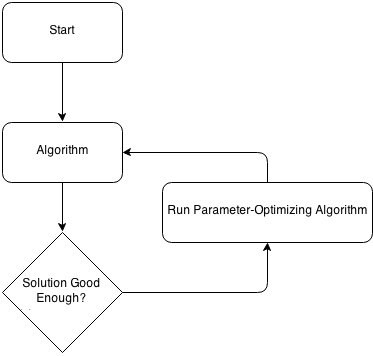
\includegraphics[scale=0.55]{./Figures/distributed_timetabling.png}
		\rule{35em}{0.5pt}
	\caption[Simplified model of a distributed timetabling for timetabling]{Simplified model of a timetabling framework}
	\label{fig:distributed_timetabling}
\end{figure}

Figure \ref{fig:distributed_timetabling} presents the framework model. The box algorithm represents any algorithm that is ready to compute a solution and if the resulting solution is not good enough (according to some criteria) a parameter-optimization-algorithm is run in order to find a better configuration. This process can iterate many times until a good solution is found.\\
This framework supports a wide range of algorithms such as Evolutionary Algorithms, Branch-and-Bound, Tabu Search and Simulated Annealing methods, runs on Windows and Linux Platforms and is implemented in JAVA, which consists of a server (JBOSS) a middle-ware (Hibernate) and a persistence engine (SQL-database). The computations are also distributed over the network using JAVA RMI technology.

\subsection{On-line Timetabling Software}
Florent Devin and Yannick Le Nir \citep{online_tt_patat2010} developed a user friendly solution using advanced technologies in the area of Rich Internet Application (RIA) and constraint programming in order to compute the timetable.


The constraints are then modeled in a constraint programming model, which requires specifying the variables, domains and constraints that constraint the assignment of variables and is implemented in swig-prolog. Web services are used to communicate with the user interface (implemented using RIA) and the communication with the database is made using a classic ODBC. 

The user interface is developed using RIA, with the ZK JAVA framework. RIA is a technology that does not require any installation on the client and it is inherently distributed, allowing users of the timetabler engine to specify constraints in a rich interface. An interesting aspect of this system is the distinction of roles, i.e., there is the normal user and the administrator. The normal user may suggest and add new constraints and the administrator will accept or refuse these new constraints. In this case, an user is someone who is allowed to submit new constraints to his own timetable.\\
In terms of persistence of the data, it is used a central shared database which is accessible by the RIA interface and the Prolog engine through Hibernate and a classical ODBC, respectively. \\
This system shows a modern approach using the advantages of RIA for data acquisition and constraint programming to compute the timetables.

\subsection{The Diamant System}

At University of Sherbrooke, the research group developed a open-source system \footnote{\href{https://github.com/gonr1001/diamant}{https://github.com/gonr1001/diamant}} capable of automatically produce class and exam timetables \citep{diamant}. Essentially the system is divided into two parts:
\begin{itemize}
	\item A module that reads data from the database and formats it according to Diamant requirements (e.g., events, students, instructors, rooms, etc).
	\item A module capable of producing timetables. This module is implemented in JAVA and follows the MVC pattern. The model contains the set of events, instructors, rooms, students and the current state of the timetable. The views give the visual representation of the sets and the timetable and reflect any changes made to the model. The controllers create a bridge between the views and the model. They control the actions sent from the view to the model, updating both parts. It is important to note that this implementation follows the open-closed principle, which means the software entities (the original classes, methods) are closed to modification but open for extension. This design pattern allows customization without modifying the source code. This system also encapsulates the algorithms with interfaces and thus allowing different implementations. 
\end{itemize}

The fact that this system is extensible, allows institutions to adapt the software to their specific needs.
%----------------------------------------------------------------------------------------
\subsection{Summary of the Features}

The presented solutions share some common characteristics and differ and innovate in others.
Table \ref{tab:summary_tech_art} shows a summary of the features presented and how these relate with the timetabling engine.

\begin{table}[H]
\centering
\resizebox{\textwidth}{!}{%
\begin{tabu}{|c|c|c|c|c|c|c|c|c|}
\hline
\multirow{2}{*}{\backslashbox{Feature}{System}} & \multirow{2}{*}{Leeds} & \multirow{2}{*}{Purdue} & \multirow{2}{*}{Bullet} & \multirow{2}{*}{THOR} & \multirow{2}{*}{\shortstack{Distributed\\ Timetabling}} & \multirow{2}{*}{\shortstack{On-line\\ Timetabling}} & \multirow{2}{*}{Diamant} & \multirow{2}{*}{\shortstack{Timetabling\\ Engine}}\\

	& & & & & & & &  \\
\hline
	Persistent Database & \ccheck & \xcheck & \xcheck & \ccheck & \ccheck & \ccheck& \ccheck & \ccheck \\
\hline
	User Interface & \xcheck& \ccheck & \ccheck & \ccheck & \xcheck & \ccheck & \ccheck & \xcheck\\
\hline
	Solver & \ccheck & \ccheck & \ccheck & \ccheck & \ccheck & \ccheck & \ccheck & \ccheck \\
\hline
	Interactive Changes & \xcheck & \ccheck & \ccheck & \ccheck& \xcheck & \xcheck&\xcheck & \xcheck\\
\hline
	Input Validation & \ccheck & \ccheck & \ccheck & \ccheck & \ccheck & \ccheck & \ccheck & \ccheck \\
\hline
	Flexibility in Preferences & \ccheck & \ccheck & \ccheck & \ccheck& \ccheck & \ccheck & \ccheck & \ccheck \\
\hline
	Distinction of Roles & \xcheck & \xcheck & \xcheck& \xcheck & \xcheck & \ccheck & \xcheck& \xcheck \\
\hline
\end{tabu}%
}
\caption[Summary of the software features]{Summary of the software features}
\label{tab:summary_tech_art}
\end{table}


